\documentclass{beamer}

%% \documentclass[handout]{beamer}
%% % use this with the [handout] option to create handouts for the audience
%% \usepackage{pgfpages}
%% \pgfpagesuselayout{2 on 1}[a4paper,border shrink=5mm]

\mode<presentation>
{
  \usetheme{Diku}
  % set this to your preferences:
  % \setbeamercovered{invisible}
  \setbeamercovered{transparent}
}

\usepackage{graphicx}
\usepackage{epic}

\usepackage{amsmath}
\usepackage{amssymb}
\usepackage{amsthm}

\newcommand{\basetop}[1]{\vtop{\vskip-1ex\hbox{#1}}}
\newcommand{\source}[1]{\let\thefootnote\relax\footnotetext{\scriptsize\textcolor{kugray1}{Source: #1}}}

% for coloured code citation in text:
\usepackage{fancyvrb}

%%%%%%%%%%%%%%%%%%%%%%%%%%%%%%%%%
%%%%% code sections   %%%%%%%%
%%%%%%%%%%%%%%%%%%%%%%%%%%%%%%%%%

% code highlighting commands in own block
\DefineVerbatimEnvironment{code}{Verbatim}{fontsize=\scriptsize}
\DefineVerbatimEnvironment{icode}{Verbatim}{fontsize=\scriptsize}

% Fancy code with color commands:
\DefineVerbatimEnvironment{colorcode}%
{Verbatim}{fontsize=\scriptsize,commandchars=\\\{\}}

%%%%%%%%%%%%%%%%%%%%%%%%%%%%%%%%%%
%%%%% some coloring    %%%%%%%%

% use "DIKU green" from our color theme for \emph
\renewcommand{\emph}[1]{\textcolor{structure}{#1}}
% use some not-too-bright red for an \emp command
\definecolor{DikuRed}{RGB}{130,50,32}
\newcommand{\emp}[1]{\textcolor{DikuRed}{ #1}}
\definecolor{CosGreen}{RGB}{10,100,70}
\newcommand{\emphh}[1]{\textcolor{CosGreen}{ #1}}
\definecolor{CosBlue}{RGB}{55,111,122}
\newcommand{\emphb}[1]{\textcolor{CosBlue}{ #1}}
\definecolor{CosRed}{RGB}{253,1,1}
\newcommand{\empr}[1]{\textcolor{CosRed}{ #1}}

\newcommand{\mymath}[1]{$ #1 $}
\newcommand{\myindx}[1]{_{#1}}
\newcommand{\myindu}[1]{^{#1}}

\newcommand{\myalt}{~|~}

\newcommand{\LO}{$\mathcal{L}_0$}


%%%%%%%%%%%%%%%%%%%%

\title{A T2 Graph-Reduction Approach To Fusion}

\author[T.Henriksen,C.Oancea]{Troels Henriksen {\tt athas@sigkill.dk}\\Cosmin Oancea {\tt cosmin@diku.dk}}

\institute{Department of Computer Science (DIKU)\\University of Copenhagen}


\date[09/23]{09/2013 \textsc{FHPC} '13}


\begin{document}

\titleslide

\begin{frame}[fragile]
  \tableofcontents
\end{frame}


%%%%%%%%%%%%%%%%%%%%%%%%%%%%%%%%%%%%%%%%%%%%%%%%%%%%%%%%%%%%%%%%%%%%%%

\section{The \LO{} language}

\subsection{First-order fragment}

\begin{frame}[fragile,t]
  \frametitle{The \LO{} Language}

  Pure, functional and quite boring.

  \begin{colorcode}
    fun int fact(int n) =
    if n = 0 then 1 else n * fact(n-1)
  \end{colorcode}

  \pause

  \begin{itemize}
  \item Primitive types: {\tt int}, {\tt char}, {\tt real}, {\tt bool}.
  \item Arrays written as {\tt \{x, y, z, ...\}}; tuples as {\tt (x, y,
      z, ...)}
  \item Arrays can be multi-dimensional, and are always regular.
  \item Built-in operations: {\tt split}, {\tt concat}, {\tt zip}, {\tt
      unzip}, {\tt transpose}, etc.
  \item Everything is fully monomorphic.
  \item Type annotations required to prevent the need for type
    reconstruction.
  \end{itemize}
\end{frame}

\begin{frame}[fragile,t]
  \frametitle{Tuples}

  No real pattern-matching (all branching is done with {\tt if}), but
  patterns for extracting tuple elements.

  \begin{colorcode}
    let (a, (b, c)) = f(x) in
    ...
  \end{colorcode}

  Tuples can contain anything, and can be elements of arrays.  During
  compilation, we convert arrays of tuples to tuples of arrays, and
  flatten all tuples.

  \pause

  \begin{itemize}
  \item {\tt (x,(y,z))} becomes {\tt (x,y,z)}.
  \item Arrays of tuples are in a sense merely syntactic sugar for
    tuples of arrays; the type {\tt [(int, real)]} is transformed to
    {\tt ([int], [real])}.
  \end{itemize}

\end{frame}

\begin{frame}
  \frametitle{Tuples, continued}

  Not always an isomorphism: {\tt [([int], [real])]}, is transformed to
  {\tt([[int]], [[real]])}.  The latter has more stringent demands to
  the regularity of arrays.  For example,

  {\tt\{(\{1\}, \{1.0\}), (\{2, 3\}, \{2.0\})\}}

  is a value of the former, but the first
  element of the corresponding transformed tuple

  {\tt(\{\{1\}, \{2, 3\}\}, \{\{1.0\}, \{2.0\}\})}

  is not a regular array.

  Hence, when determining whether a program generates regular arrays, we
  must look at the \textit{transformed} values - in a sense, the
  regularity requirement ``transcends'' the tuples.  Also, after
  tuple-transformation, {\tt zip} and {\tt unzip} disappear.

\end{frame}

\begin{frame}[fragile,t]
  \frametitle{Do-loops}

  \LO{} supports sequential do-loops with a special syntax.\\
  \hfill\\
  \begin{block}{Loop to recursive function}
    \begin{minipage}{0.2\columnwidth}
      \begin{colorcode}
loop (x = a) =
  for i < n do
    \emp{g(x)}
in \emph{body}
      \end{colorcode}
    \end{minipage}
    \pause
    \begin{minipage}{0.05\columnwidth}
      $\Rightarrow$
    \end{minipage}
    \begin{minipage}{0.1\columnwidth}
      \begin{colorcode}
fun t f(int i, int n, t x) =
  if i >= n
    then x
    else f(i+1, n, \emp{g(x)})

let x = f(i, n, a)
in \emph{body}
      \end{colorcode}
    \end{minipage}
  \end{block}

  Where {\tt t} is the type of {\tt x}.

  (A little more complicated in practice, as {\tt g(x)} may be an
  expression containing free variables.)

\end{frame}

\begin{frame}[fragile,t]
  \frametitle{In-place updates}

  Let-with construct used to update slices of arrays.

  \begin{colorcode}
    let b = a with [i\mymath{\myindx{1}},...,i\mymath{\myindx{k}}] <- v
    in body
  \end{colorcode}

  \pause

  \begin{block}{Fibonacci function}
    \begin{colorcode}
fun [int] main(int n) =
  let res = replicate(n, 1) in
  loop (res) = for i < n-2 do
    let res <- res with [i+2] = res[i] + res[i+1] in
    res
  in res
    \end{colorcode}
  \end{block}

  We would like to modify the array {\em in-place} while maintaining
  referential transparency.

\end{frame}

\begin{frame}[fragile,t]
  \frametitle{In-place updates part 2: Uniqueness types}

  We can do this by aliasing analysis and {\em uniqueness types}.

  \begin{colorcode}
    let b = a with [i\mymath{\myindx{1}},...,i\mymath{\myindx{k}}] <- v
    in body
  \end{colorcode}

  Acceptable iff {\tt a} (or any of its aliases) are not used
  afterwards, and it is not alised to a {\it non-unique} function
  parameter.

  \begin{colorcode}
    fun \emp{*}[int] computefibs(\emp{*}[int] arr) =
      let n = size(arr) in
      let arr[0] = 1 in
      let arr[1] = 1 in
      loop (arr) = for i < n-2 do
        let x = arr[i] in
        let y = arr[i+1] in
        let arr[i+2] = x + y in
        arr
      in arr
  \end{colorcode}

  The {\tt *} denotes a {\em unique} value.  Unique arguments are not
  used after the call, and unique return values are not aliased to any
  of the function parameters.

\end{frame}

\subsection{Second-order array combinators}

\begin{frame}[fragile,t]
  \frametitle{Second-order array combinators (SOACs)}

  All higher-order functions are built in.

  \begin{block}{Built-in higher order functions}
    {\tt map($f$, $e_{1}$, \ldots, $e_{n}$)} \\
    {\tt filter($f$, $e_{1}$, \ldots, $e_{n}$)} \\
    {\tt reduce($f$, $x_{1}$, \ldots, $x_{n}$, $e_{1}$, \ldots, $e_{n}$)} \\
    {\tt scan($f$, $x_{1}$, \ldots, $x_{n}$, $e_{1}$, \ldots, $e_{n}$)} \\
    {\tt redomap($f_{r}$, $f_{m}$, $x_{1}$, \ldots, $x_{n}$, $e_{1}$, \ldots, $e_{n}$)} \\
  \end{block}

  We assume that all tuples are flat and passed element-wise - e.g., if
  the accumulator to {\tt reduce} is a tuple, $x_{1}$, \ldots, $x_{n}$
  is its components.
\pause
\\\hfill\\
  {\tt map(f, a, b) = unzip(map'(f', zip(a,b)))}


\end{frame}

\begin{frame}[fragile,t]
  \frametitle{{\tt redomap}}

  {\tt redomap($f_{r}$, $f_{m}$, $x_{1}$, \ldots, $x_{n}$, $e_{1}$, \ldots, $e_{n}$)}

  Not part of the external language, but useful for the fusion
  algebra.  Semantics is the same as\\{\tt foldl($f_{m}$, $(x_{1},\ldots,x_{n})$, zip($e_{1}$, \ldots, $e_{n}$))}.
\pause
\begin{block}{List homomorphism} {\tt (red $\odot$ e) . (map f)} can
  be transformed to:  \\
  ${\tt red}\mbox{ }\odot\mbox{ }{\tt e}\mbox{ }.\mbox{ }{\tt
    map}\mbox{ }{\tt f}\mbox{ }\emphh{\equiv}$ $\mbox{ }{\tt
    red}\mbox{ }\odot\mbox{ }{\tt e}\mbox{ }.\mbox{ }{\tt pmap}_{p}
  \mbox{ }$ $(\emp{{\tt red} \mbox{
    }\odot\mbox{ }{\tt e}\mbox{ }.\mbox{ }{\tt map}\mbox{ }{\tt f}})$\\
  Hence the {\em inner} map-reduce can be
  rewritten as a left-fold:\\
  ${\tt red}\mbox{ }\odot\mbox{ }{\tt e}\mbox{ }.\mbox{ }{\tt
    map}\mbox{ }{\tt f}\mbox{ }\emphh{\equiv}$ $\mbox{ }{\tt
    red}\mbox{ }\odot\mbox{ }{\tt e}\mbox{ }.\mbox{ }{\tt pmap}_{p}
  \mbox{ }$ $(\emp{{\tt foldl}\mbox{
    }{\tt g}\mbox{ }{\tt e}})$\\
  It follows that in order to be generate parallel code for \\
  {\tt (red $\odot$ e) . (map f)} we need to record either $\odot$ and
  {\tt f}, or $\odot$ and {\tt g}. We chose the latter, i.e., {\tt
    redomap($\odot$, g, e)}, because it allows a richer compositional
  algebra for fusion.  In particular, it allows to fuse {\tt reduce
    $\circ$ map $\circ$ filter} into a {\tt redomap} without
  duplicating computation.
\end{block}

\end{frame}

\section{Conservative Fusion}

\begin{frame}[fragile,t]
  \frametitle{What Not To Fuse?}

  Currently, the rules are:

  \begin{itemize}
  \item ``DON'T fuse if changes program semantics'' (common sense)
  \item ``DON'T fuse if computation is duplicated'' (modulo negligible?)
  \end{itemize}

  \bigskip

  Examples:
  \begin{itemize}
  \item Don't fuse inside a loop from outside (\texttt{noFusion1})\\
    (might change asymptotic complexity) \smallskip

  \item Don't fuse if you compute an array twice (\texttt{noFusion2})\smallskip

  \item Currently, don't fuse even if it intuitively negligible (\texttt{noFusion3})\smallskip

  \item Don't fuse if it is incorrect. (\texttt{noFusion3})
  \end{itemize}

\end{frame}

\begin{frame}[fragile,t]
  \frametitle{Example: In-Place Array Update Restrictions}

  \begin{block}{Incorrect Fusion (because of the in-place semantics)}
    \begin{center}
      \begin{colorcode}[fontsize=\scriptsize]
fun real main([real] arr) =
let x      = map(f, arr)  in
let arr[1] = 3.33         in
let y      = map(g, x)    in
y[0]
      \end{colorcode}
      $\Downarrow$
      \begin{colorcode}[fontsize=\scriptsize]
fun real main([real] arr) =
let arr[1] = 3.33            in
let y      = map(g . f, arr) in
y[0]
      \end{colorcode}
    \end{center}
  \end{block}
\end{frame}

\begin{frame}[fragile,t]
  \frametitle{Example: Fusing into a loop}

  \begin{block}{Inefficient Fusion (because of work duplication)}
\begin{center}
      \begin{colorcode}[fontsize=\scriptsize]
fun real main([real] a, [[real]] b) =
let x      = map(f, a)                 in
let y      = map(fn real ([real] v) =>
                 map(h,x,v), b)        in
y[0]
      \end{colorcode}
$\Downarrow$
      \begin{colorcode}[fontsize=\scriptsize]
fun real main([real] a, [[real]] b) =
let y      = map(fn real ([real] v) =>
                 map(\mymath{combine(f,h)},a,v), b) in
y[0]
      \end{colorcode}
\end{center}
  \end{block}
\end{frame}

\section{Simple Fusion}

\begin{frame}[fragile,t]
  \frametitle{What Can We Fuse?}

  \begin{block}{Simple Fusion Example}\vspace{-1ex}
    \begin{columns}
      \column{0.3\textwidth}\vspace{-1ex}
      \begin{colorcode}[fontsize=\scriptsize]
fun real f(real a) = a + 3.0
fun real g(real a) = a * 3.0

fun real main([real] arr) =
  let x = map(f, arr) in
  let y = map(g, x)   in
  let z = map(g, y)   in
  z[0]
      \end{colorcode}
      \column{0.45\textwidth}
      \begin{colorcode}[fontsize=\scriptsize]
fun real main([real] arr) =
  let z = map(fn real (real a) =>
                let b = a + 3.0 in
                let c = b * 3.0 in
                c * 3.0, arr) in
  z[0]
      \end{colorcode}
    \end{columns}
  \end{block}

\end{frame}
\begin{frame}[fragile,t]
  \frametitle{What Can We Fuse?}
  \begin{block}{Simple Fusion Example (Cont)}
\begin{center}
    \begin{colorcode}[fontsize=\scriptsize]
fun real f(real a) = a + 3.0
fun real h1(real a, real b, real c) = a * b + c
fun real h2(real a, real b) = a * b
fun real main([real] arr) =
  let x = map(f, arr) in
  let y = map(f, arr) in
  let z = if arr[0] < 0.0
            then map(h1, x, y, x)
            else map(h2, y, x) in
  z[0]
    \end{colorcode}
$\Downarrow$
    \begin{colorcode}
fun real main([real] arr) =
  let z =
    if arr[0] < 0.0 then
      map(fn real (real a) => (a + 3.0) * (a + 3.0) + (a + 3.0), arr)
    else map(fn real (real a) => (a + 3.0) * (a + 3.0), arr_4)
  in z[0]
    \end{colorcode}
\end{center}
  \end{block}
\end{frame}


\section{Discussion}
\begin{frame}[fragile,t]
  \frametitle{``Related Work''}

  \emp{Seems like everybody does fusion, but the explanations w.r.t. how are not very comprehensive.}

  \bigskip
  Anonymous quote:

  \smallskip

  \emph{``Existing fusion transforms rely on inlining to move producer
    and consumer expressions next to each other, which allows
    producer/consumer pairs to be detected. However, when let-bound
    variables are used multiple times in the body of an expression,
    un- restrained inlining can lead to duplication of work. Compilers
    such as GHC, handle this situation by only inlining the
    definitions of let- bound variables that have a single use site,
    or by relying on some heuristic about the size of the resulting
    code to decide what to inline ''}

\end{frame}


\begin{frame}[fragile,t]
  \frametitle{How About This One?}

  Arrays \texttt{y1, y2, y3, z1, z2} are used multiple times .... \\ \emp{so we shouldn't fuse?}

  \begin{block}{How About This one}
    \begin{colorcode}[fontsize=\scriptsize]
      fun (real,real,real) f1( real a1, real a2 ) =
        (a1 * a2, a1 + a2, a1 - a2)

      fun (real,real)      f2( real a1, real a2 ) =
        (a1 - a2, a1 + 2.0*a2)

      fun (real,real)      g ( real a1, real a2, real a3, real a4 ) =
        (a1 * a2 - a3 * a4, a3 + a4 + a2 - a1)

      fun real myop ( real a1, real a2, real a3, real a4, real a5 ) =
        a1+a2+a3+a4+a5

      fun real main([real] x1, [[real]] x2) =
        let (y1, y2, y3) = map( f1, x1, x2[1] )        in
        let (z1, z2)     = map( f2, y1, y2 )           in
        let (q1, q2)     = map( g , y3,z1,y2,y3 )      in
        let res          = map( myop, q1,q2,z2,y1,y3 ) in
        res[3]
    \end{colorcode}
  \end{block}

\end{frame}

\begin{frame}[fragile,t]
  \frametitle{T1-T2 Transform?}

If repeated application of T$_1$ and T$_2$ to a control-flow graph ({\sc cfg})
results in one point, then the {\sc cfg} is said to be reducible, i.e.,
the code can be re-written using only regular (while) {\tt loop}s,
{\tt if} and {\tt goto}-free statements (with function calls).

  \vbox{
    \begin{center}
      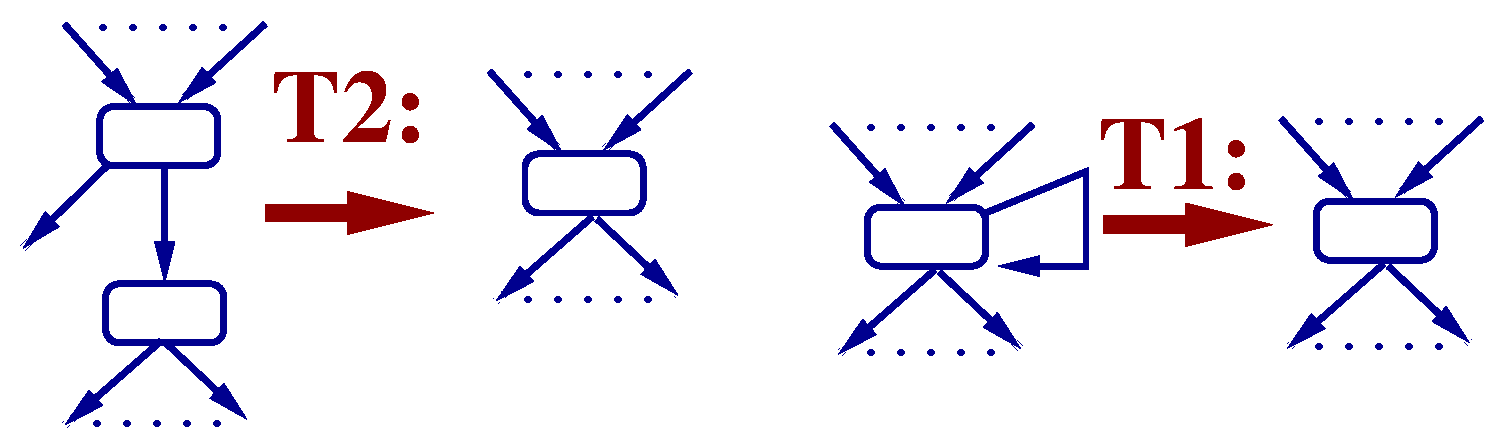
\includegraphics[height=17ex]{Figures/CFG_T12}
    \end{center}
  }

\LO{} guarantees reducible {\sc cfg}.

\end{frame}

\begin{frame}[fragile,t]
  \frametitle{T1-T2 Transform!}

\vbox{
\begin{minipage}{0.46\columnwidth}
\begin{center}
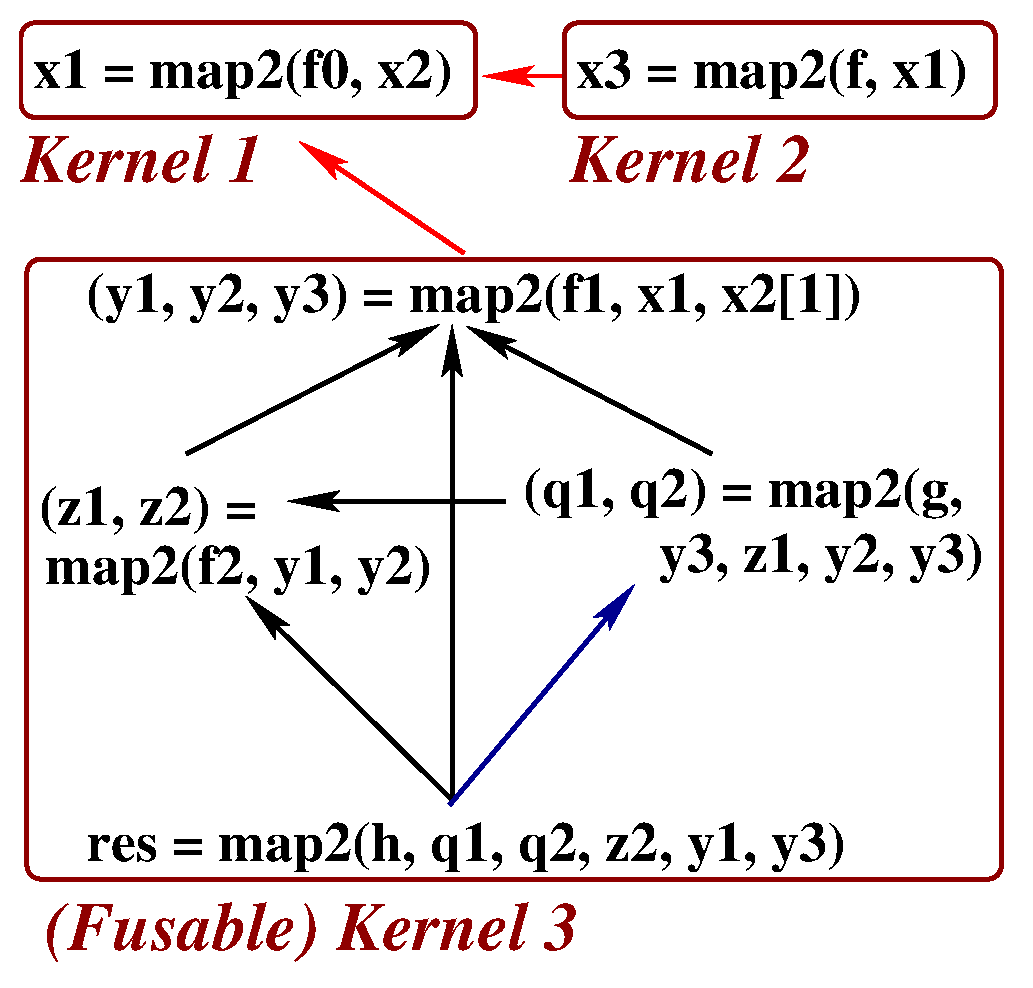
\includegraphics[height=30ex]{Figures/T1T2}
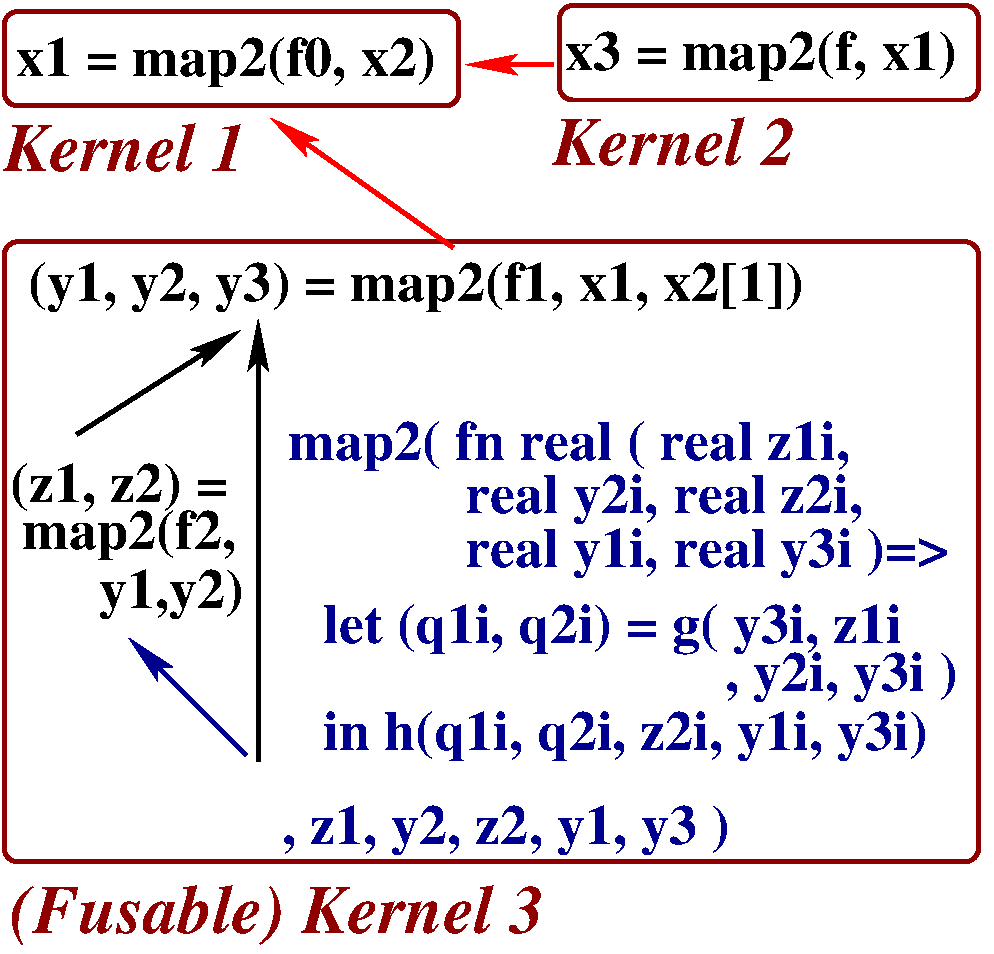
\includegraphics[height=30ex]{Figures/T1T2Fuse1}
\end{center}
\end{minipage}
}
Replace inputs {\tt q1}, {\tt q2} with {\tt y3, z1, y2, y3}, removing
duplicates.
\end{frame}

\begin{frame}[fragile,t]
  \frametitle{T1-T2 Transform!, continued}

\vbox{
\begin{minipage}{0.46\columnwidth}
\begin{center}
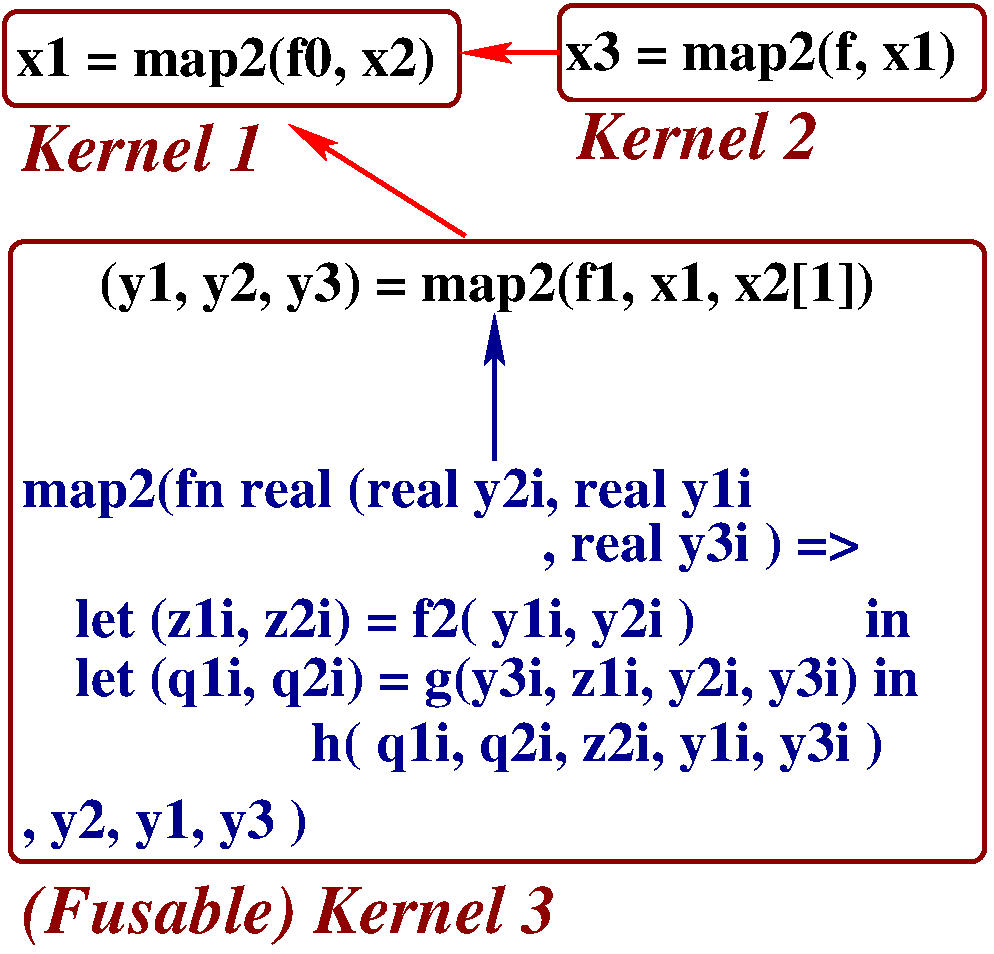
\includegraphics[height=30ex]{Figures/T1T2Fuse2}
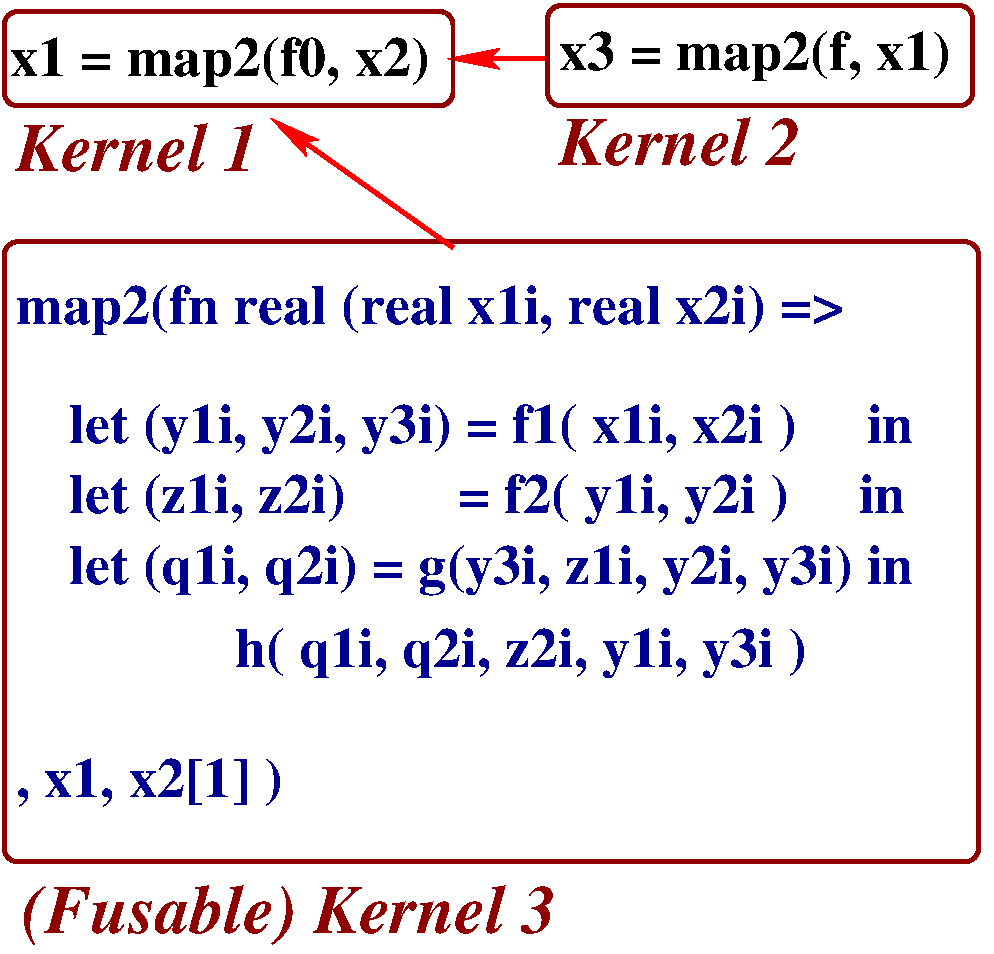
\includegraphics[height=30ex]{Figures/T1T2Fuse3}
\end{center}
\end{minipage}
}
\end{frame}

\begin{frame}[fragile,t]
  \frametitle{Technicalities}

  We assume a normalised program.  This means we do not have to build
  the data-dependency graph explicitly, as a bottom-up traversal is
  guaranteed to encounter the SOACs in the proper order.

  The implementation is somewhat complex, but all bookkeeping, so I'll
  skip the details.

  \begin{itemize}
    \item About 700 lines of Haskell.
    \item ``Fast enough''.
    \item Fully intraprocedural, relies on aggressive inlining.
  \end{itemize}
\end{frame}

\begin{frame}[fragile,t]
  \frametitle{Fusion algebra}

\vbox{
\begin{minipage}{0.48\columnwidth}
\begin{colorcode}
// \emp{replicate can be fused}
//\emp{without restrictions}
let x = replicate(N,a)in
let y = map(f, x, b) in
let z = map(g, x, c) in
let x[i] = ...
    \emphh{\mymath{\equiv}}
let x = replicate(N, a) in
let y = map( fn \mymath{\beta\myindx{1}} (\mymath{\alpha\myindx{1}} b\mymath{\myindx{i}})
              => f(a,b\mymath{\myindx{i}}), b)
let z = map( fn \mymath{\beta\myindx{2}} (\mymath{\alpha\myindx{2}} c\mymath{\myindx{i}})
              => g(a,c\mymath{\myindx{i}}), c)
in let x[i] = ...


//\emp{map o map \mymath{\Rightarrow} map}
let (x1, x2) = map(f, a1)
in  map(g, x1, y)
    \emphh{\mymath{\equiv}}
map(fn \mymath{\beta} (\mymath{\alpha\myindx{1}} a1\mymath{\myindx{i}}, \mymath{\alpha\myindx{2}} y\mymath{\myindx{i}})
  =>let (x1\mymath{\myindx{i}}, x2\mymath{\myindx{i}}) = f(a1\mymath{\myindx{i}})
    in  g(x1\mymath{\myindx{i}}, y\mymath{\myindx{i}})
, a1, y )
\end{colorcode}
\end{minipage}
\hfill
\begin{minipage}{0.48\columnwidth}
\begin{colorcode}
//\emp{filter o filter\mymath{\Rightarrow}filter}
//\emp{{\em{}IFF} consumer's input set}
//\emp{  \mymath{\subseteq} producer's output set}
let (x1,x2)=filter(c\mymath{\myindx{1}},a1,a2)
in  let y = filter(c\mymath{\myindx{2}}, x1) ..
    \emphh{\mymath{\equiv}}
let (y, dead) = filter(
  fn bool (\mymath{\alpha\myindx{1}} a1\mymath{\myindx{i}},\mymath{\alpha\myindx{2}} a2\mymath{\myindx{i}})=>
      if   c\mymath{\myindx{1}}(a1\mymath{\myindx{i}}, a2\mymath{\myindx{i}})
      then c\mymath{\myindx{2}}(a1\mymath{\myindx{i}})
      else false
, a1, a2 ) ..

//\emp{reduce o filter\mymath{\Rightarrow}reduce}
//\emp{{\em{}IFF} consumer's input set}
//\emp{  \mymath{\equiv} producer's output set}
let x = filter(c, a)
in  reduce(\mymath{\oplus}, e, x)
    \emphh{\mymath{\equiv}}
reduce(fn \mymath{\beta} (\mymath{\beta} e, \mymath{\beta} a\mymath{\myindx{i}}) =>
  if c(a\mymath{\myindx{i}}) then \mymath{\oplus}(e,a\mymath{\myindx{i}}) else e
, e, a )
\end{colorcode}
\end{minipage}
}
\end{frame}

\begin{frame}[fragile,t]
  \frametitle{Fusion algebra, continued}

\vbox{
\begin{minipage}{0.48\columnwidth}
\begin{colorcode}
//\emp{reduce o map\mymath{\Rightarrow}redomap}
let (x1, x2) = map(f, a1)
in  reduce(\mymath{\oplus},e\mymath{\myindx{1}},e\mymath{\myindx{2}}, x1,y)
    \emphh{\mymath{\equiv}}
redomap(\mymath{\oplus}
, fn (\mymath{\beta\myindx{1}},\mymath{\beta\myindx{2}}) ( \mymath{\beta\myindx{1}} e\mymath{\myindx{1}}, \mymath{\beta\myindx{2}} e\mymath{\myindx{2}}
             , \mymath{\alpha\myindx{1}} a1\mymath{\myindx{i}},\mymath{\alpha\myindx{2}} y\mymath{\myindx{i}})
   => let (x1\mymath{\myindx{i}}, x2\mymath{\myindx{i}}) = f(a1\mymath{\myindx{i}})
      in  \mymath{\oplus}(e\mymath{\myindx{1}},e\mymath{\myindx{2}},x1\mymath{\myindx{i}},y\mymath{\myindx{i}})
, (e\mymath{\myindx{1}}, e\mymath{\myindx{2}}), a1, y )


//\emp{redomap o map\mymath{\Rightarrow}redomap}
let (x1, x2) = map(f, a1)
in  redomap(\mymath{\oplus}, g, e, x1, y)
    \emphh{\mymath{\equiv}}
redomap(\mymath{\oplus}
, fn \mymath{\beta} (\mymath{\beta} e, \mymath{\alpha\myindx{1}} a1\mymath{\myindx{i}}, \mymath{\alpha\myindx{2}} y\mymath{\myindx{i}})
   => let (x1\mymath{\myindx{i}}, x2\mymath{\myindx{i}}) = f(a1\mymath{\myindx{i}})
      in  g(e, x1\mymath{\myindx{i}}, y\mymath{\myindx{i}})
, e, a1, y )
\end{colorcode}
\end{minipage}
\hfill
\begin{minipage}{0.48\columnwidth}
\begin{colorcode}
//\emp{reduce o filter\mymath{\Rightarrow}redomap}
//\emp{{\em{}IFF} consumer's input set}
//\emp{  \mymath{\subseteq} producer's output set}
let (x1,x2)=filter(c, a1, a2)
in  reduce(\mymath{\oplus}, e, x1)
    \emphh{\mymath{\equiv}}
redomap(\mymath{\oplus}
, fn \mymath{\beta} (\mymath{\beta} e, \mymath{\alpha\myindx{1}} a1\mymath{\myindx{i}}, \mymath{\alpha\myindx{2}} a2\mymath{\myindx{i}})
   => if c(a1\mymath{\myindx{i}}, a2\mymath{\myindx{i}})
      then \mymath{\oplus}(e, a1\mymath{\myindx{i}}) else e
, e, a1, a2 )

//\emp{redomap o filter\mymath{\Rightarrow}redomap}
//\emp{{\em{}IFF} consumer's input set}
//\emp{  \mymath{\subseteq} producer's output set}
let (x1,x2)=filter(c, a1, a2)
in  redomap(\mymath{\oplus}, g, e, x1)
    \emphh{\mymath{\equiv}}
redomap(\mymath{\oplus}
, fn \mymath{\beta} (\mymath{\beta} e, \mymath{\alpha\myindx{1}} a1\mymath{\myindx{i}}, \mymath{\alpha\myindx{2}} a2\mymath{\myindx{i}})
   => if c(a1\mymath{\myindx{i}}, a2\mymath{\myindx{i}})
      then g(e, a1\mymath{\myindx{i}}) else e
, e, a1, a2 )
\end{colorcode}
\end{minipage}
}
\end{frame}

\begin{frame}[fragile,t]
  \frametitle{Finally ... }

  Always fuse \emph{replicate} as it does not duplicates computation.

  \bigskip

\begin{colorcode}
fun   int    redplus1( [int]  a) = reduce(op +, 0, a)
fun  [int]   redplus2([[int]] a) = map   (redplus1, a)

fun  [int]   mul1( [int]  a,  [int]  b) = map(op *, a, b)
fun [[int]]  mul2([[int]] a, [[int]] b) = map(mul1, a, b)

fun [[int]]  replin(int N, [int] a) = replicate(N, a)

fun [[int]] main(int N, [[int]] a, [[int]] b ) =
    let br  = replicate( N, transpose(b) ) in
    let ar  = map      ( replin(N),    a ) in
    let abr = map  (mul2, ar, br)          in
        map(redplus2, abr)
\end{colorcode}
\end{frame}

\begin{frame}[fragile,t]
  \frametitle{Finally ... }

\begin{colorcode}
fun [[int]] main(int N, [[int]] a, [[int]] b ) =
    let br  = replicate( N, transpose(b) ) in
    let ar  = map      ( replin(N),    a ) in
    let abr = map  (mul2, ar, br)      in
        map(redplus2, abr)
\end{colorcode}

Fuses to...

\begin{colorcode}
fun [[int]] main(int N, [[int]] a, [[int]] b) =
  let br = transpose(b) in
  map(fn [int] (int i, [int] r) =>
      map(fn int (int j, [int] c) =>
          redomap(fn int (int x, int y) => x + y,
                  fn int (int x, int y) => x * y,
                  0, r, c),
          iota(N), br),
      iota(N), a)
\end{colorcode}

\end{frame}

\begin{frame}[fragile, t]
\frametitle{Fusion hindrances}

\begin{colorcode}
let \emphh{x} = map2(f, a)      in    let n = size(a)/2      in
let n = size(\emp{x})/2       in    let (a\mymath{\myindx{1}},a\mymath{\myindx{2}})=split(n,a) in
let (\emphh{x\mymath{\myindx{1}}},\emphh{x\mymath{\myindx{2}}})=split(n,\emp{x})  in \mymath{\Rightarrow} let \emphh{x\mymath{\myindx{1}}} = map2(f, a\mymath{\myindx{1}})   in
let y = reduce2(g,\emphh{x\mymath{\myindx{1}}},\emphh{x\mymath{\myindx{2}}})..    let \emphh{x\mymath{\myindx{2}}} = map2(f, a\mymath{\myindx{2}})   in
                              let y = reduce2(g,\emphh{x\mymath{\myindx{1}}},\emphh{x\mymath{\myindx{2}}})..
\end{colorcode}
The use of {\tt x} in {\tt size} and {\tt split} in the lefthand-side
code would inhibit fusion.
\end{frame}

\begin{frame}[fragile,t]
  \frametitle{Experiments}

{\tiny
\begin{center}
\begin{tabular}{l|c|c|c|c|c|c}
Fusion Statistics & P0 & P1 & P2 & P3 & P4 & P5 \\\hline
Lines Of Code          & 283 & 859 & 182 & 23 & 19 & 22\\\hline\hline
{\tt map} $\circ$ {\tt map}          & 10 & 1  & 8  & 5 & 3  &   \\\hline
{\tt map} $\circ$ {\tt replicate}    &    &    & 12 & 2 & 2  &   \\\hline
{\tt redomap} $\circ$ {\tt filter}   & 1  &    &    &   &    &   \\\hline
{\tt redomap} $\circ$ {\tt map}      & 5  &    &    &   &    &   \\\hline
{\tt reduce} $\circ$ {\tt map}       & 6  & 12 &    & 2 & 1  & 1 \\\hline
{\tt reduce} $\circ$ {\tt replicate} &    & 3  &    &   &    &   \\\hline\hline
Interesting            &    & 1  & 1  &   &    &   \\\hline
\end{tabular}
\end{center}
}

\begin{description}
%\begin{itemize}
\item[P0:] a real-world pricing kernel for financial derivatives.
\item[P1:] a real-world market calibration kernel that computes some
  of the parameters of P0.
\item[P2:] a real-world kernel for stochastic volatility calibration
  via Crank-Nicolson finite differences solver.
\item[P3:] a flat-parallelism, array-based implementation of the
  shortest-path algorithm,
\item[P4:] flat-parallelism implementation of matrix multiplication.
\item[P5:] an implementation of the maximal segment sum problem.
%\end{itemize}
\end{description}

\end{frame}

\section{Conclusions and future work}

\begin{frame}[fragile,t]
\frametitle{Future work: ISWIM}

The fusion algebra for {\tt scan} and {\tt reduce} is relatively poor.
The Interchange Scan With Inner Maps ({\sc iswim}) transform helps.

\begin{colorcode}
scan( fn [real] ([real] x, [real] y) => map(op +, x, y),
     , {0.0,..,0.0}, a )
transpose( map(fn [real] ([real] x) => scan(op +,0.0,x)
         , transpose(a) )
\end{colorcode}
\pause
We can generalise {\tt transpose} and {\tt map} to multiple
dimensions.

\begin{colorcode}
// \emp{Generalization for nested map (similar for reduce)}
map\mymath{\myindu{1}}(f, a\mymath{\myindx{1}},.., a\mymath{\myindx{k}}) \emphh{\mymath{\equiv}} map(g, a\mymath{\myindx{1}},.., a\mymath{\myindx{k}})
map\mymath{\myindu{n}}(f, a\mymath{\myindx{1}},.., a\mymath{\myindx{k}}) \emphh{\mymath{\equiv}} map(fn ([\mymath{\beta\myindx{1}}],..,[\mymath{\beta\myindx{t}}]) ([\mymath{\alpha\myindx{1}}] x\mymath{\myindx{1}},..,[\mymath{\alpha\myindx{k}}] x\mymath{\myindx{k}}) =>
                            map\mymath{\myindu{n-1}}(f, x\mymath{\myindx{1}},.., x\mymath{\myindx{k}}) , a\mymath{\myindx{1}},.., a\mymath{\myindx{k}} )

// \emp{Generalization for transpose}:
b=transpose(k,n,a) \mymath{\Rightarrow} a[i\mymath{\myindx{1}},..,i\mymath{\myindx{k}},i\mymath{\myindx{k+1}},..,i\mymath{\myindx{k+n}},..,i\mymath{\myindx{q}}] \emphh{\mymath{\equiv}}
                      b[i\mymath{\myindx{1}},..,i\mymath{\myindx{k+1}},..,i\mymath{\myindx{k+n}},i\mymath{\myindx{k}},..,i\mymath{\myindx{q}}]

// \emp{Fusing across transpose}:
let x=map\mymath{\myindu{n}}(f,a) in let y=transpose(1,n-k,x) in map\mymath{\myindu{n}}(g,y)
        \emphh{\mymath{\equiv}} map\mymath{\myindu{n}}(g o f, transpose(1,n-k,a) )
\end{colorcode}

\end{frame}

\begin{frame}[fragile,t]
\frametitle{Future work: ISWIM, continued}

Arbitrary-nested-level generalisation of {\sc iswim}.

\begin{colorcode}
\emp{scan}( fn ( [\mymath{\myindx{1}}[\mymath{\myindx{..n}}\mymath{\alpha\myindx{1}}]],    .., [\mymath{\myindx{1}}[\mymath{\myindx{..n}}\mymath{\alpha\myindx{k}}]] )
          ( [\mymath{\myindx{1}}[\mymath{\myindx{..n}}\mymath{\alpha\myindx{1}}]] x\mymath{\myindu{1}\myindx{1}}, .., [\mymath{\myindx{1}}[\mymath{\myindx{..n}}\mymath{\alpha\myindx{k}}]] x\mymath{\myindu{1}\myindx{k}},
            [\mymath{\myindx{1}}[\mymath{\myindx{..n}}\mymath{\alpha\myindx{1}}]] x\mymath{\myindu{2}\myindx{1}}, .., [\mymath{\myindx{1}}[\mymath{\myindx{..n}}\mymath{\alpha\myindx{k}}]] x\mymath{\myindu{2}\myindx{k}} ) =>
                \emphh{map}\mymath{\myindu{n}}(\mymath{\oplus}, x\mymath{\myindu{1}\myindx{1}},..., x\mymath{\myindu{1}\myindx{k}}, x\mymath{\myindu{2}\myindx{1}},..., x\mymath{\myindu{2}\myindx{k}})
     , ne\mymath{\myindx{1}}, ..., ne\mymath{\myindx{k}}, a\mymath{\myindx{1}}, ..., a\mymath{\myindx{k}}) \emphh{\mymath{\equiv}}
let (..., re\mymath{\myindx{t}}, ...) = (..., map\mymath{\myindu{n}}( replicate(1), ne\mymath{\myindx{t}} ), ...) in
// replicate dim n of neutral elems so map sizes match
let ( y\mymath{\myindx{1}},.., y\mymath{\myindx{k}} ) =
  \emphh{map} (fn ( [\mymath{\myindx{1}}[\mymath{\myindx{..n}}\mymath{\alpha\myindx{1}}]], ..., [\mymath{\myindx{1}}[\mymath{\myindx{..n}}\mymath{\alpha\myindx{k}}]] )
           ( [\mymath{\myindx{1}}[\mymath{\myindx{..n}}\mymath{\alpha\myindx{1}}]] x\mymath{\myindx{1}}, ..., [\mymath{\myindx{1}}[\mymath{\myindx{..n}}\mymath{\alpha\myindx{k}}]] x\mymath{\myindx{k}} ) =>
          \emphh{map}\mymath{\myindu{n-1}}( fn ([\mymath{\myindx{1}}[\mymath{\myindx{..n-1}}\mymath{\alpha\myindx{1}}]],  ..., [\mymath{\myindx{1}}[\mymath{\myindx{..n-1}}\mymath{\alpha\myindx{k}}]] )
                      ([\mymath{\myindx{1}}[\mymath{\myindx{..n-1}}\mymath{\alpha\myindx{1}}]] e\mymath{\myindx{1}},..,[\mymath{\myindx{1}}[\mymath{\myindx{..n-1}}\mymath{\alpha\myindx{k}}]] e\mymath{\myindx{k}},
                       [\mymath{\myindx{1}}[\mymath{\myindx{..n-1}}\mymath{\alpha\myindx{1}}]] x\mymath{\myindx{1}},..,[\mymath{\myindx{1}}[\mymath{\myindx{..n-1}}\mymath{\alpha\myindx{k}}]] x\mymath{\myindx{k}})
                     => \emp{scan}(\mymath{\oplus}, e\mymath{\myindx{1}}[0],..,e\mymath{\myindx{k}}[0], x\mymath{\myindx{1}},..,x\mymath{\myindx{k}})
                 , re\mymath{\myindx{1}}, ..., re\mymath{\myindx{k}}, x\mymath{\myindx{1}}, ..., x\mymath{\myindx{k}} )
       , transpose(1,n,a\mymath{\myindx{1}}), ..., transpose(1,n,a\mymath{\myindx{k}}) )
in (transpose(n, q\mymath{\myindx{1}}-n, y\mymath{\myindx{1}}), ..., transpose(n, q\mymath{\myindx{k}}-n, y\mymath{\myindx{k}}))
// transpose back the result; q\mymath{\myindx{t}}-n is the dimension of \mymath{\alpha\myindx{t}}
\end{colorcode}

\end{frame}

\begin{frame}[fragile,t]
  \frametitle{Conclusions}

  We can fuse even somewhat complex dataflow - particularly, when
  producer/consumer output/input sets to do match exactly.

  No good experimental results yet.

  \pause
  \begin{itemize}
    \item Wild applause
    \item Spontaneous rioting by the crowd
    \item Questions?
  \end{itemize}

\end{frame}


\end{document}
